\chapter{Schedule Comparison}
\label{chap:Comparison}
\section{Expected Cost Comparison}
Suppose that there are $N$ customers to be scheduled. In the case of the static schedule, the optimal policy is given by $\mathbf{x}_{N}^{*} = (x_{1}^{*}, \ldots, x_{N - 1}^{*})$ and the expected cost of the optimal policy is given by $\phi (\mathbf{x}_{N}^{*})$. In the case of the dynamic schedule, the initial state is $(N, 0)$, so the expected cost of the optimal policy is given by $C_{N}^{*} (0)$.

Clearly, as the dynamic schedule has the ability to match the optimal policy for the static schedule, $C_{N}^{*} (0) \leq \phi (\mathbf{x}_{N}^{*})$ (i.e., the dynamic schedule cannot have greater expected cost) regardless of the number of customers to be scheduled. As found in Chapter~\ref{chap:Dynamic}, equality is attained for the cases where $N \in \{ 0, 1, 2 \}$ as the schedules are identical in those cases.

Figure~\ref{Graph_Cost_Comparison} plots the expected costs of both schedules against the number of customers to be scheduled ($N$) assuming $\gamma = 0.5$ and $\mu = 1$.
\begin{figure}[htb]
	\centering
	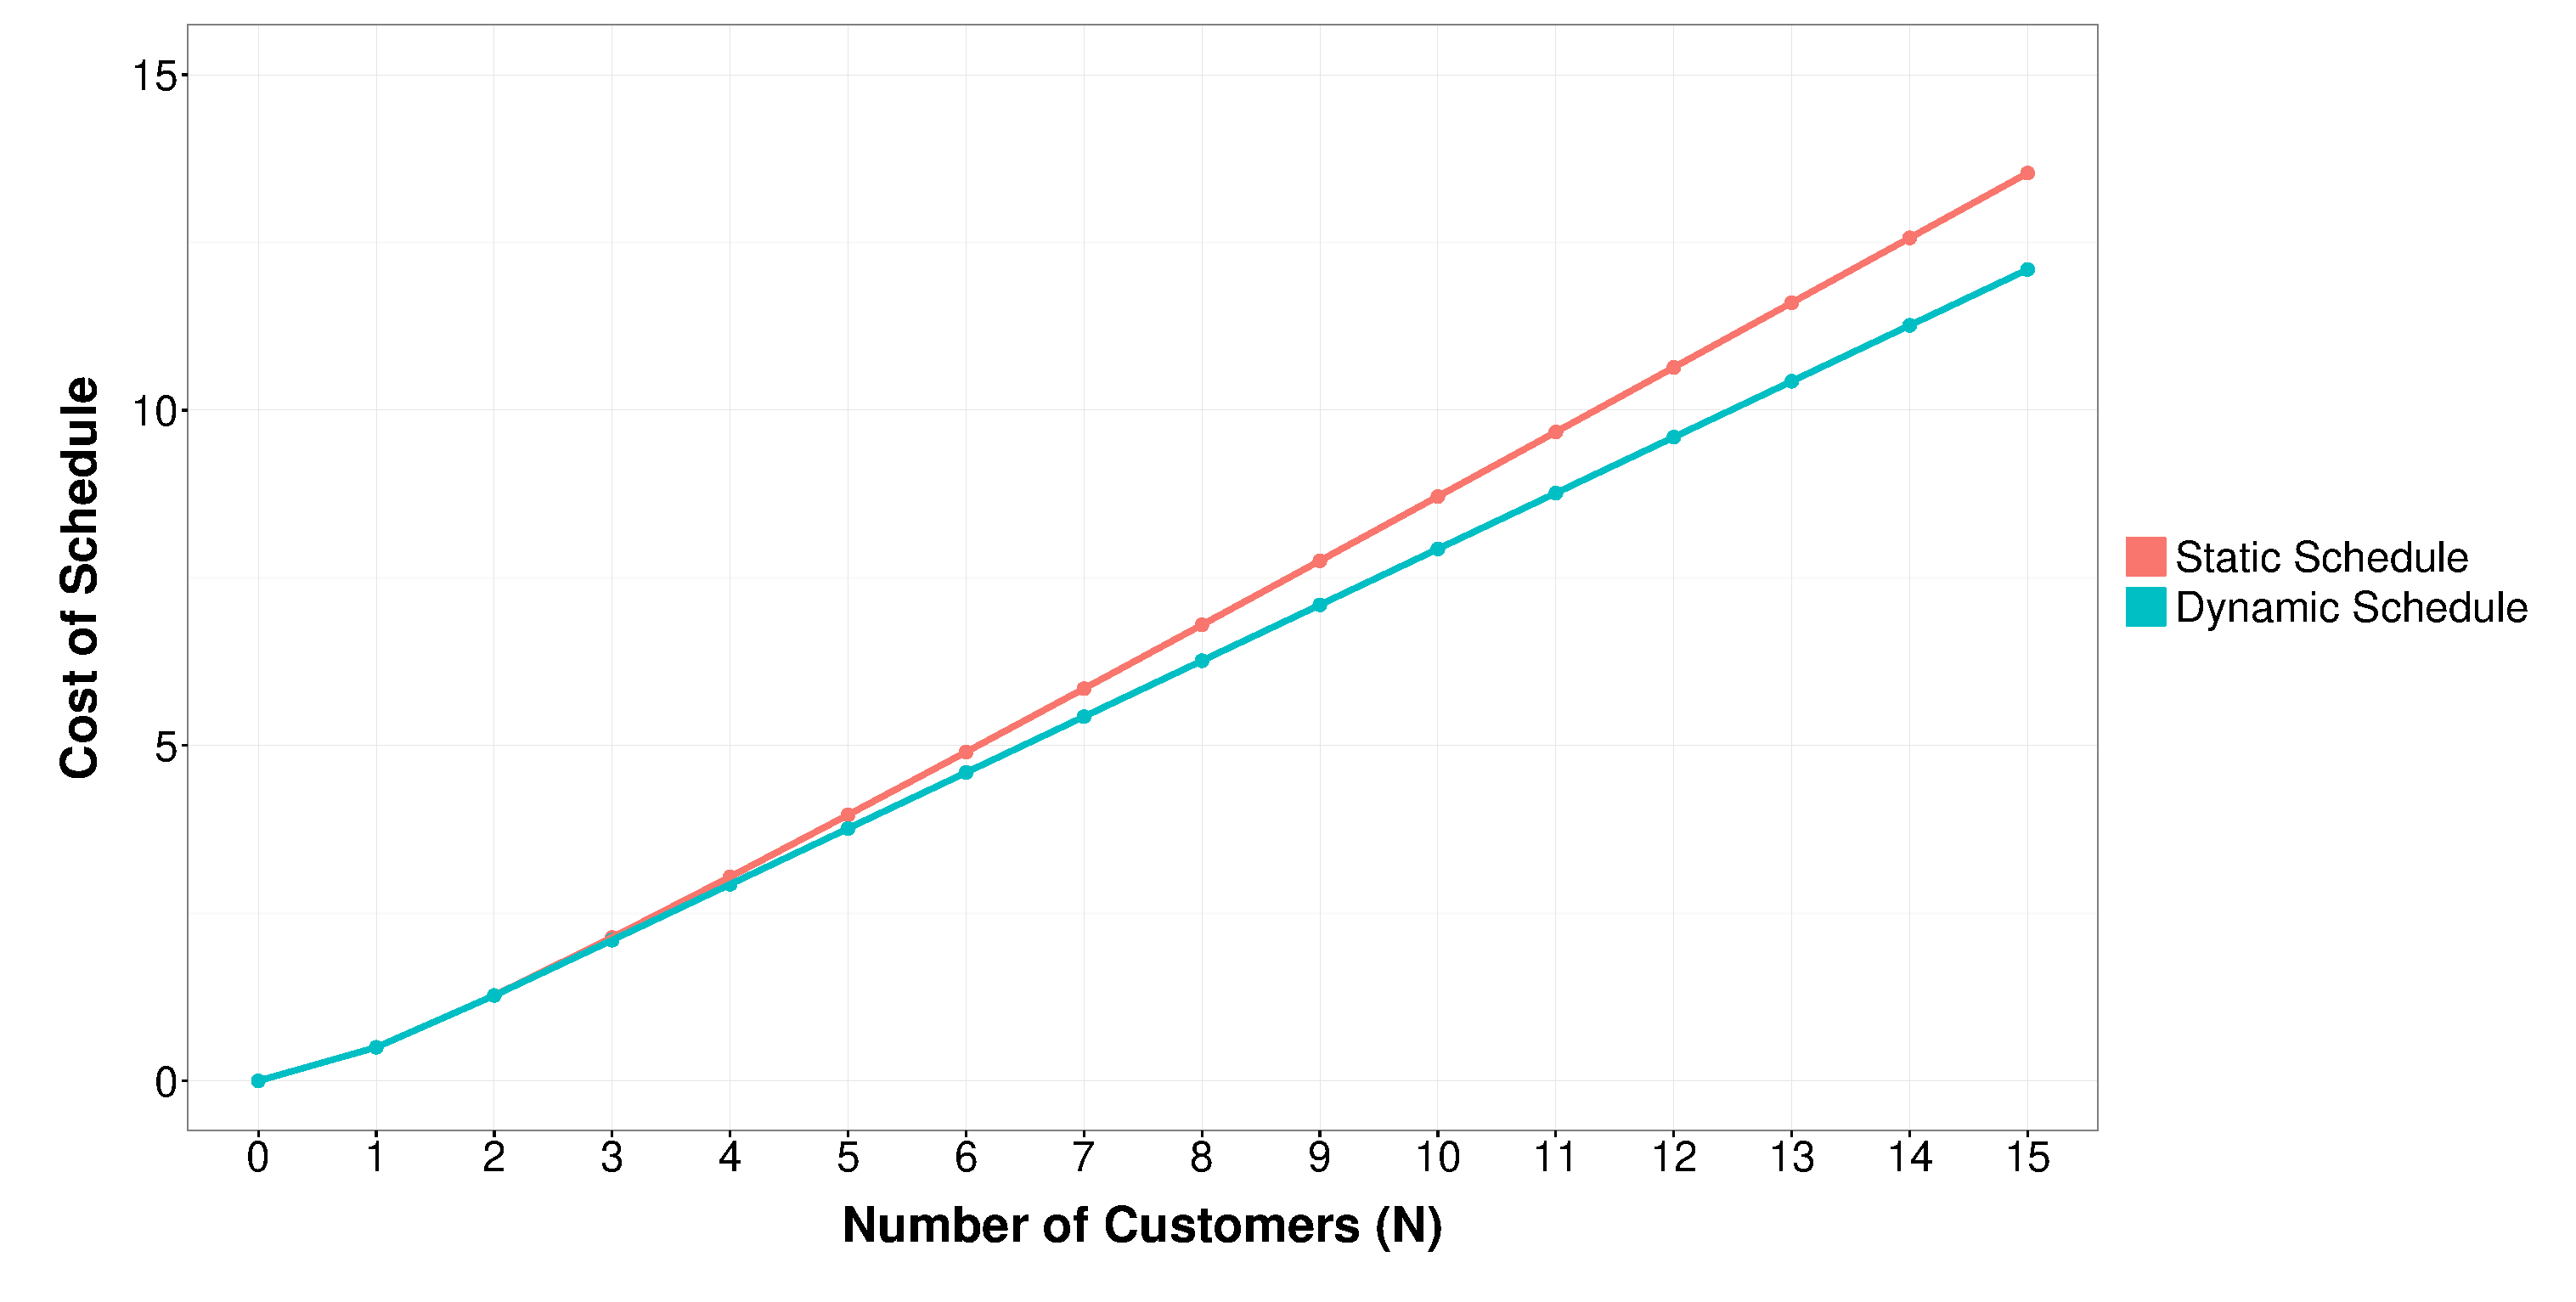
\includegraphics[width = 0.85\textwidth]{Comparison_Line_Cost_Num.eps}
	\caption{Plot of the expected cost of each schedule against the number of customers to be scheduled ($N$) for both the static and dynamic schedules where $N \in \{ 0, \ldots, 15 \}$, $\gamma = \frac{c_{S}}{c_{S} + c_{W}} = 0.5$ and $\mu = 1$.}
	\label{Graph_Cost_Comparison}
\end{figure}

As expected, the costs are identical for $N \in \{ 0, 1, 2 \}$. For all other $N$ values, the cost of the static schedule is greater than the cost of the dynamic schedule. The cost difference appears to be minimal for $N \leq 5$, but as $N$ increases the cost difference increases.

\section{Expected Percentage Cost Saving}
Define the expected percentage cost saving $\Delta C$ (i.e., the percentage difference between the expected cost of the static schedule and the dynamic schedule) as
\begin{equation}
	\Delta C \coloneqq 100 \times \frac{\phi (\mathbf{x}_{N}^{*}) - C_{N}^{*} (0)}{\phi (\mathbf{x}_{N}^{*})}.
\end{equation}

Figure~\ref{Graph_Cost_Saving} plots the percentage cost saving ($\Delta C$) against $\gamma$ for various values of the number of customers ($N$) to be scheduled. 
\begin{figure}[htb]
	\centering
	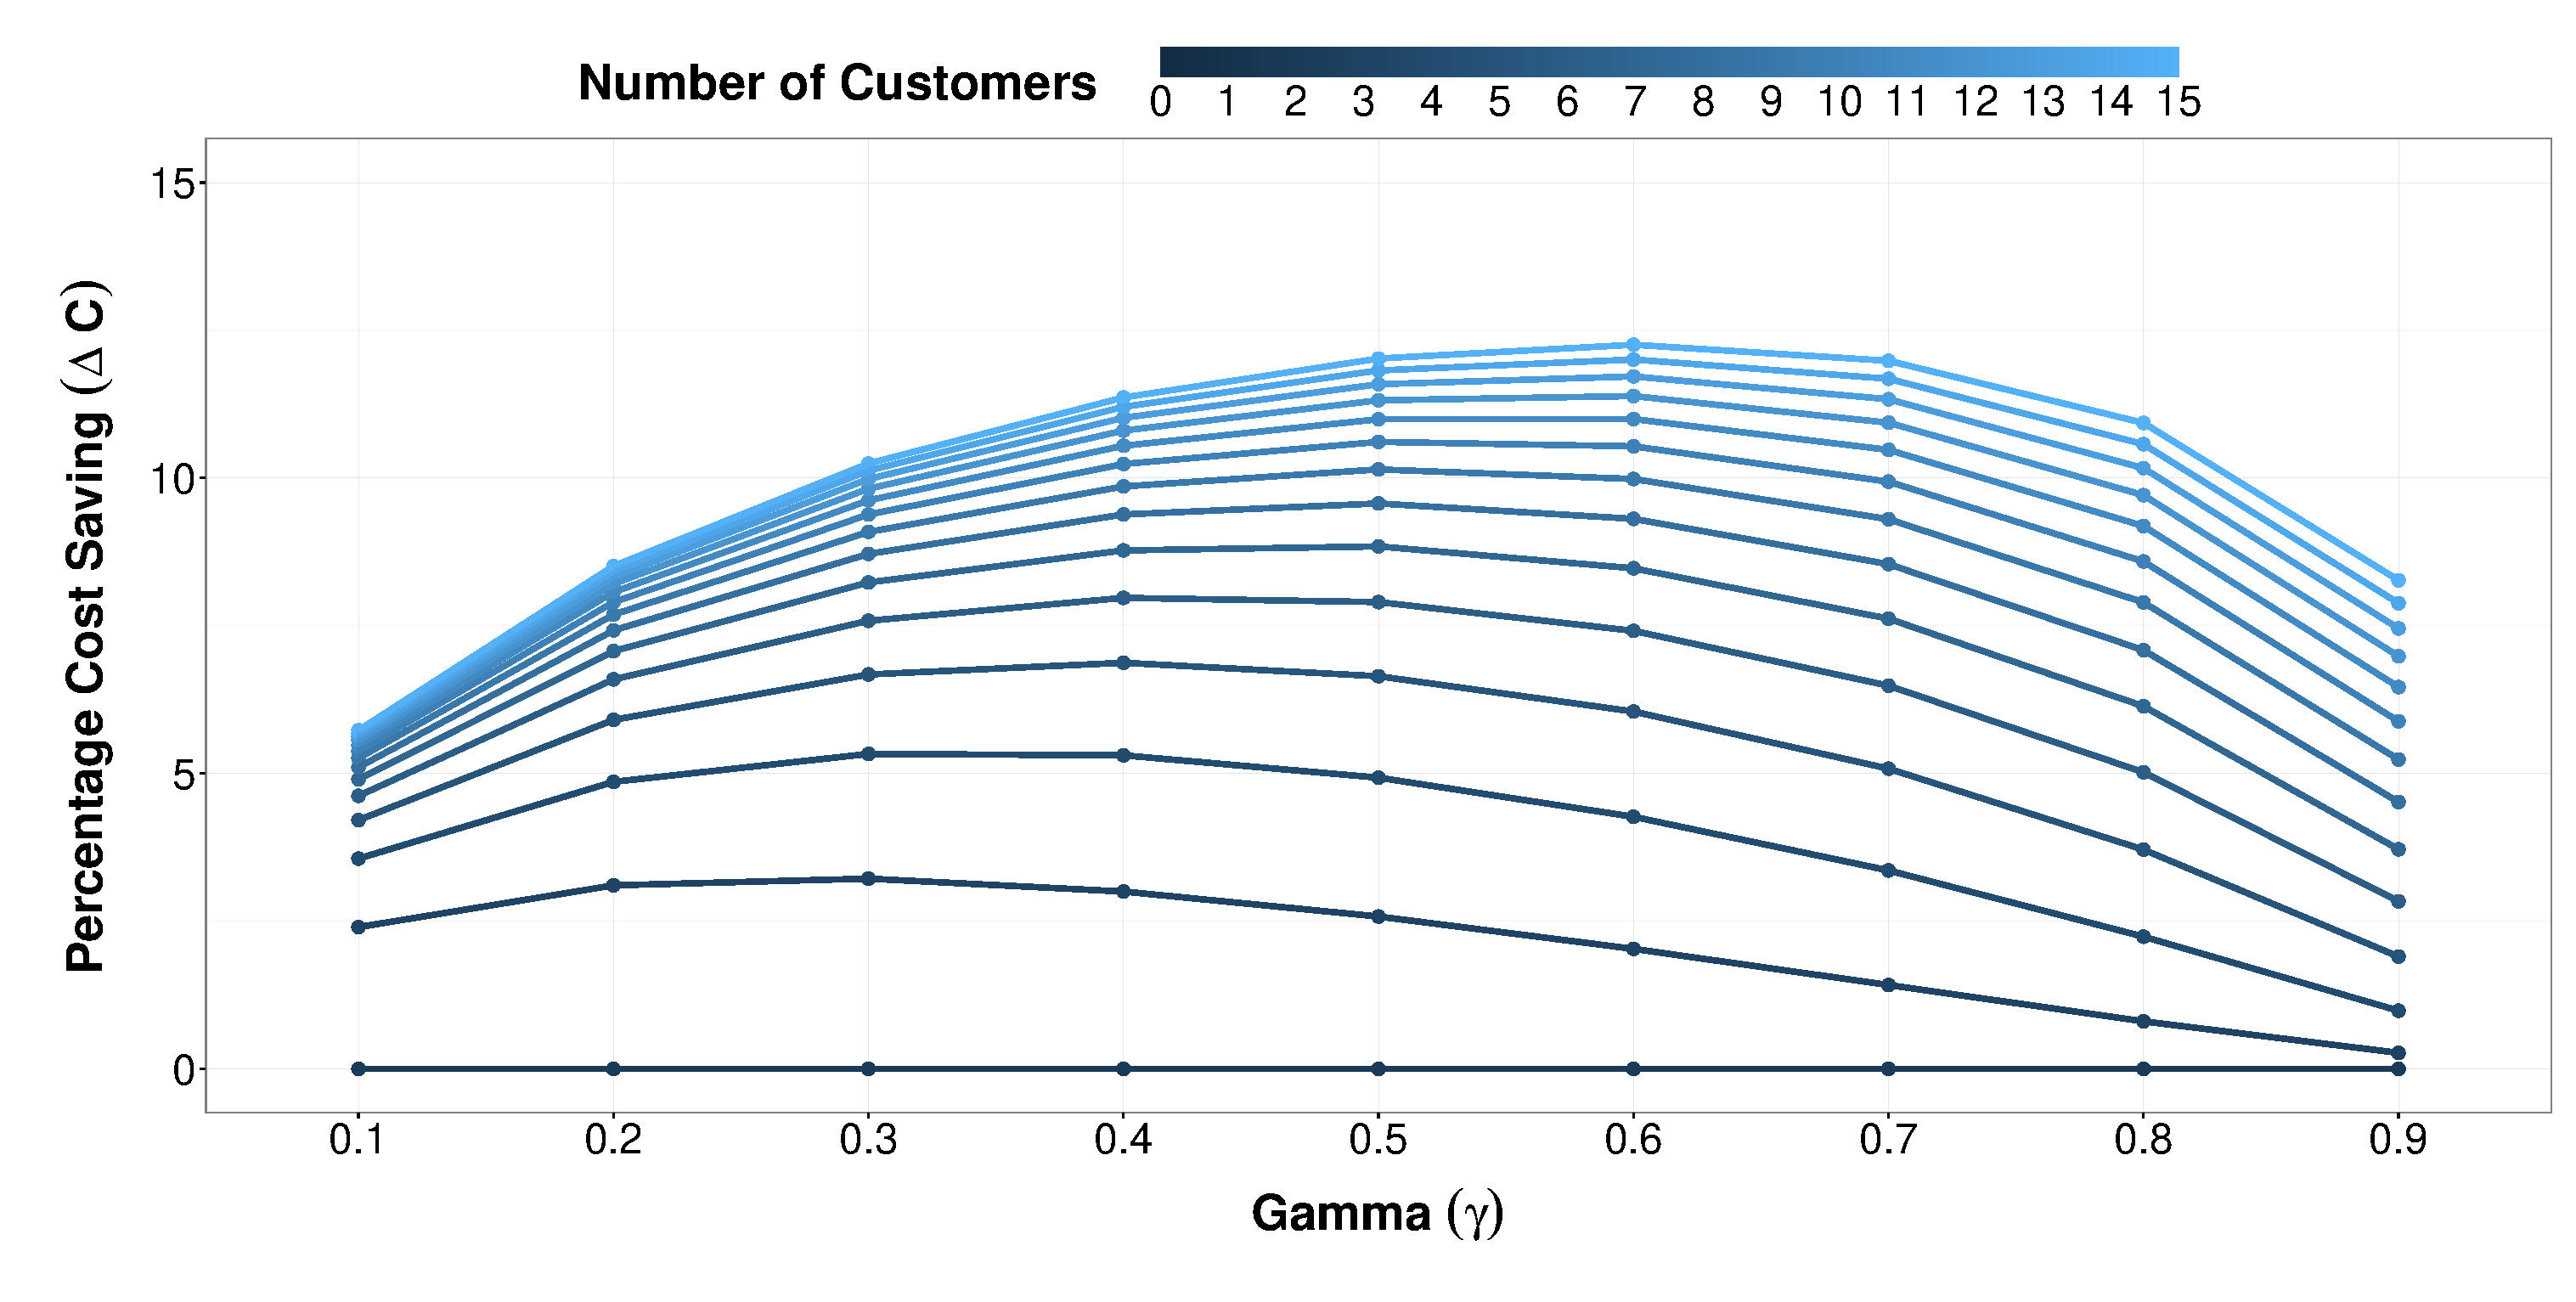
\includegraphics[width = 0.85\textwidth]{Cost_Saving_Line_Num.eps}
	\caption{Plot of the percentage cost saving ($\Delta C$) against $\gamma = \frac{c_{S}}{c_{S} + c_{W}}$ where $N = \{ 0, \ldots, 15 \}$ and $\mu = 1$.}
	\label{Graph_Cost_Saving}
\end{figure}

For $N \in \{ 0, 1, 2 \}$, $\Delta C = 0$ for all values of $\gamma$ as the schedules are identical. As $N$ increases with $\gamma$ held constant, $\Delta C$ increases as the dynamic schedule begins to outperform the static schedule. $\Delta C$ increases at a decreasing rate (i.e., the curves become closer together as $N$ increases). The maximal value of $\Delta C$ is $10.6 \%$. Even if $N$ were to increase further beyond $15$, it does not appear that the expected percentage cost saving would exceed $15 \%$.

$\Delta C$ is at a minimum for the extreme values of $\gamma$ (i.e., $\gamma = 0.1$ and $\gamma = 0.9$). An extreme value of $\gamma$ indicates that the either the customer waiting cost or the server availability cost is a significant priority (i.e., $c_{W} \gg c_{S}$ or $c_{S} \gg c_{W}$). If one of the costs is heavily prioritised, there is little difference between the static and dynamic schedules, thus $\Delta C$ is small.

For each value of $N \geq 3$, the peak value of $\Delta C$ occurs at a middle value of $\gamma$. As $N$ increases, the peak occurs at a larger value of $\gamma$. For $N = 3$ the peak occurs at $\gamma = 0.3$, whereas for $N = 15$ the peak occurs at $\gamma = 0.7$.

The difference between the dynamic and static schedule is most significant for middle values of $\gamma$ (e.g., $\gamma \in [0.4, 0.7]$). For $\gamma = 0.1$, it doesn't appear that the expected percentage cost saving would exceed $5 \%$ indicating very little difference between the schedules.